\documentclass[a4paper,10pt]{article}

\usepackage{epsfig}
\usepackage{subfigure}
\usepackage{calc}
\usepackage{amssymb}
\usepackage{amstext}
\usepackage{amsmath}
\usepackage{amsthm}
\usepackage{multicol}
\usepackage{pslatex}
\usepackage{natbib}
\let\cite\citep
%%%% nasty hack to get rid of conflict of an annoying conflict
\makeatletter
\let\bibhang\@undefined
\makeatother
%%%% 
\usepackage{apalike}
% Please add other packages that you may need BEFORE the SCITEPRESS.sty package.
\usepackage{xcolor}
%%%%%%%%%%%%%%%%%%%%%%%%%%%%%%%%%%%%%%%%%%%%%%%%%%%%%%%%%%%%%%%%%%
\usepackage{SCITEPRESS}

\subfigtopskip=0pt
\subfigcapskip=0pt
\subfigbottomskip=0pt

%%%%%%%%%%%%%%%%%%%%%%%%%%%%%%%%%%%%%%%%%%%%%%%%%%%%%%%%%%%%%%%%%%
\newcommand{\TODO}[1]{\begingroup\color{red}#1\endgroup}
\newcommand{\PFS}[1]{\begingroup\color{green}#1\endgroup}
\newcommand{\NR}[1]{\begingroup\color{orange}#1\endgroup}
\newcommand{\FK}[1]{\begingroup\color{blue}#1\endgroup}

\newcommand{\DINGENS}[1]{\texttt{DINGENS}}
\newcommand{\pprec}{\mathrel{\prec\!\!\!\prec}}
\newcommand{\SAFTWARE}{\texttt{vaPLA}} %{\TODO{\texttt{SAFTWARE}}}

\begin{document}

\title{A General Framework for Exact Partially Local Alignments}

\author{\authorname{Falco Kirchner\sup{1}, Nancy Retzlaff\sup{2,1}, and
    Peter F.\ Stadler\sup{1,2,3,4,5}} \affiliation{\sup{1}Bioinformatics
    Group, Department of Computer Science, Interdisciplinary Center for
    Bioinformatics, and Competence Center for Scalable Data Services and
    Solutions Dresden/Leipzig, Universit{\"a}t Leipzig
    H{\"a}rtelstra{\ss}e 16-18, D-04107 Leipzig,
    Germany}
  \affiliation{\sup{2}Max Planck Institute for Mathematics in
    the Sciences, Inselstra{\ss}e 22, D-04103 Leipzig, Germany}
  \affiliation{\sup{3}Institute for Theoretical Chemistry, University of
    Vienna, W{\"a}hringerstra{\ss}e 17, A-1090 Wien, Austria}
  \affiliation{\sup{4}Santa Fe Institute, 1399 Hyde Park Road, Santa Fe NM
    87501, USA} \email{FALCO@nirwana.net,
    \{nancy,studla\}@bioinf.uni-leipzig.de} }

\keywords{Multiple sequence alignments, dynamics programming} 


\TODO{R2: Link to software}

\TODO{R3: \\
3. Please place Fig. 1 in p. 3 rather than in p. 2}

\abstract{Multiple sequence alignments are a crucial intermediate step in a
  plethora of data analysis workflows in computational biology. While
  multiple sequence alignments are usually constructed with the help of
  heuristic approximations, exact pairwise alignments are readily
    computed by dynamic programming algorithms. In the pairwise case,
  local, global, and semi-global alignments are distinguished, with key
  applications in pattern discovery, gene comparison, and homology search,
  respectively. With increasing computing power, exact alignments of
  triples and even quadruples of sequences have become feasible and recent
  applications e.g.\ in the context of breakpoint discovery have shown that
  mixed local/global multiple alignments can be of practical interest.
  \SAFTWARE{} is the first implementation of partially local multiple
  alignments of a few sequences and provides convenient access to this
  family of specialized alignment algorithms.}

\onecolumn \maketitle \normalsize \vfill

\section{\uppercase{Introduction}}

\noindent
Global multiple alignments are typically constructed as intermediate data
structure to support a comparative or evolutionary analysis homologous
sequences. Alignment problems are naturally treated as optimization
problems: a scoring function evaluates the similarities in an alignment
column and/or the pattern of gaps. Multiple alignments are almost
exclusively treated globally, that is, all parts of the input sequence is
scored. The notion of ``local multiple alignments'' appears mostly in
  the context of phylogenetic footprinting \cite{Lukashin:99,Blanchette:02}
  and related pattern discovery problems \cite{Tabei:09}, where substrings
  are considered that appear with a limited number of mismatches in some or
  all input sequences.

Local variants of sequence alignment, on the one hand, play an important
role in pairwise alignments. Local alignments, i.e., maximally similar
substrings within pairs of longer sequences, are a natural way to identify
conserved domains.  The semi-global variant of pairwise alignment, in which
one sequence, usually called ``query'', is expected to appear as
approximate substring of a larger ``subject'', again is a natural
formalization of homology search, implemented e.g.\ in \texttt{gotohscan}
\cite{Hertel:09a}.  Overlap alignments \cite{Jones:04} allowing free end
gaps on all sequences have applications e.g.\ in sequence assembly
\cite{Rausch:09}. Until recently, the generalization of these variants to
more than two sequences has received very little attention.

Pairwise alignment problems can be solved exactly for a wide range of cost
models by means of dynamic programming. In fact, the algorithms of
\citet{Needleman:70} for global alignments, \citet{Smith:81} for local
alignments, and the extension to affine gap costs by \citet{Gotoh:82} are
among the early, paradigmatic example of dynamic programming. The basic
recursive structure is readily extended to more than two input sequences
\cite{Carillo:88,Lipman:89}; the time and space complexity, however, grows
exponentially with the number of sequences. Exact dynamic programming
solutions thus have been used in practice only for 3-way
\cite{Gotoh:86,Dewey:01,Konagurthu:04,Kruspe:07a} or 4-way
\cite{Steiner:11a} alignments. Since multiple sequence alignment problems
(for arbitrary numbers of input sequences $X$ are typically NP-hard
\cite{Kececioglu:93,Wang:94,Bonizzoni:01,Just:01,Manthey:03,Elias:06}, they
are solved by heuristic approximation algorithms, see
\citet{Chatzou:16}, \citet{Baichoo:17} or \citet{Nute:18} for a recent reviews.

As the exact 3-way and 4-way alignments have increased in usage, variants
of the problem that combine local and global alignments have been proposed
for specialized application scenarios. \citet{AlArab:17a} considered the
fate of sequences in the wake of mitochondrial genome rearrangements by
simultaneously comparing the rearranged region to both of its
ancestors. This approach made it possible to distinguish tandem duplication
random loss (TDRL) from reversal or transposition events. This specialized
3-way alignment problem suggested the need to develop a general theoretical
framework for alignments that consider part of their input local and part
global. As shown by \citet{Retzlaff:18a} it is possible -- and convenient
-- to allow the user determine separately for each input sequence and each
of its ends, whether it is to be treated as global, i.e., deletions of a
prefix or a suffix are penalized, or as local, allowing the omission of
prefixes or suffixes at not cost. We will briefly outline the theoretical
results in the following section. While the presentation by
\citet{Retzlaff:18a} is purely theoretical and did not supply a reference
implementation, the present contribution closes this gap.

\section{\uppercase{Theory}}

The basic idea behind the framework of \citet{Retzlaff:18a} boils down to
two ingredients: (1) Each input sequence is either local or global on the
left and either local or global on the right. This is entirely the user's
choice and provided with the input. (2) In a particular alignment column, a
sequence may be \textit{inactive} (if up to this column its prefix is
considered unaligned), \textit{active} (if it contributes to the column
either with one of its characters or with a gap this is scored), or it is
\textit{dead} (if its suffix is considered unaligned). Consequently a
left-local sequence starts out \textit{inactive}, while a left-global
sequence starts out \textit{active}. Correspondingly, a right-global input
is still \textit{active} at the end of the alignment, while a right-local
sequence must be \textit{dead} at the end of the alignment. The partially
local alignment problems can be solved by dynamic programming just as the
classic pairwise problems mentioned in the introduction. As usual, a
scoring (\emph{memoization}) table $S$ holds the optimal alignments of
prefixes. The only difference is that $S$ now depends not only on the
length of prefixes but also on the state (\textit{inactive},
\textit{active}, or \textit{dead}) of each sequence in a given column of
the alignment. It is sufficient to record the set $A$ of \textit{active}
and $D$ of \textit{dead} sequences, since the \emph{inactive} sequences are
given by $X\setminus\{A \cup D\}$.  As the alignment progresses, an
\textit{inactive} sequence may become \textit{active} only once, and an
\textit{active} may transit at most once to the \textit{dead}
state. Consecutive alignment columns thus have state pairs $(A',D')$ and
$(A,D)$ that are comparable w.r.t.\ the partial order
\begin{equation}
  (A',D')\preceq(A,D) \iff
    \begin{cases} A'\cup D'\subseteq A\cup D \\
      D'\subseteq D
    \end{cases}
\end{equation}
The state changes can be performed stepwisely. As shown by
\citet{Retzlaff:18a}, $(A',D')$ is an immediate predecessor of $(A,D)$ if
either exactly on one \textit{inactive} sequence become \textit{active} or
exactly one \textit{active} sequence transitions to the dead state.  We
denote this relation by $\pprec$. The initial condition is $A=A_0$, where
$A_0$ is the set of left-global sequences, and $D=\emptyset$.

\begin{figure}
  \begin{center}
    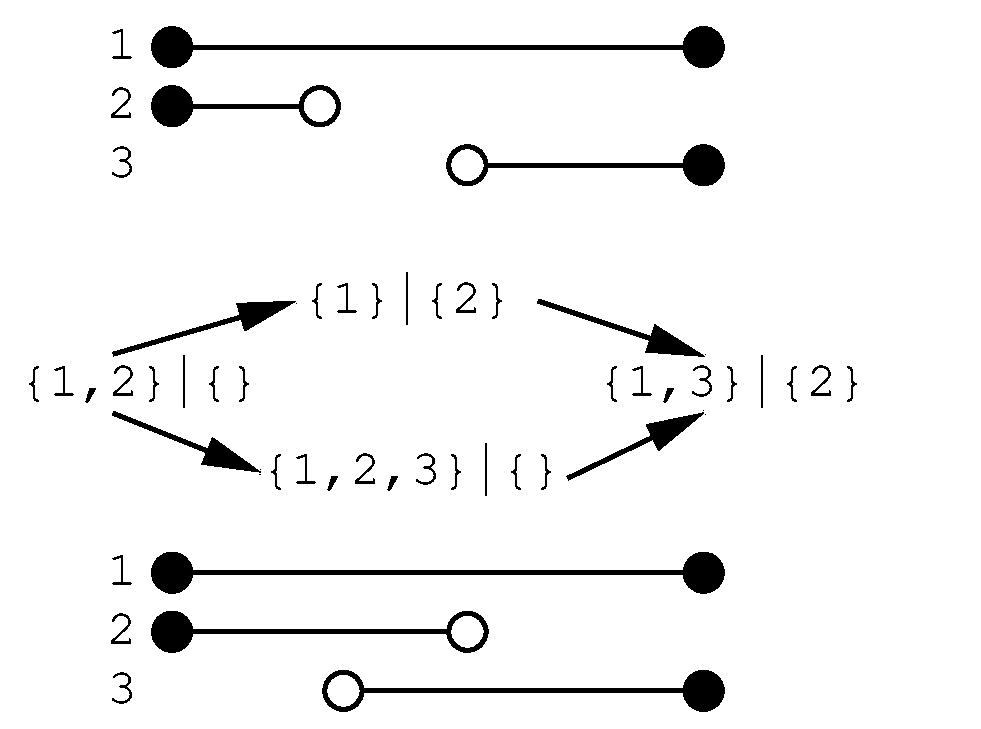
\includegraphics[width=0.9\columnwidth]{Fig1.eps}
  \end{center}
  \caption{Schematic representation of the breakpoint alignment model of
    \cite{AlArab:17a}, with global reference sequence $\mathtt{1}$,
    right-local prefix $\mathtt{2}$, and left-local suffix $\mathtt{3}$.
    The initial and terminal states of valid alignments are therefore
    $A|D=\{\mathtt{1},\mathtt{2}\}|\{\}$ and
    $\{\mathtt{1},\mathtt{3}\}|\{\mathtt{2}\}$, respectively.  There are
    two distinct path of transitioning between these states with
    intermediates states $\{\mathtt{1}\}|\{\mathtt{2}\}$ (if $\mathtt{2}$
    and $\mathtt{3}$ do not overlap) and $\{\mathtt{1,2,3}\}|\{\}$ (if
    $\mathtt{2}$ and $\mathtt{3}$ overlap in their aligned part). The black
    bullets indicate that the correspond end of the sequence is present in
    the alignment, open circles indicate the prefixes of suffixes remain
    unaligned.}
  \label{fig:Marwa}
\end{figure}

In a quite general form (which uses the heuristic version of the affine gap
cost model for more than two sequences), the recursion for the optimal
alignment score are of the form
\begin{equation} 
  S^{(A,D)}_I = \max 
      \begin{cases}
        \displaystyle\max_{\pi} 
            \left[ S^{(A,D)}_{I-\pi} + s(\pi)
                    \right]
        \\
        \displaystyle\max_{(A',D')\pprec(A,D)}  
                    \left[ S^{(A,D)}_I + s^*\right]
       \end{cases} 
\label{eq:maxrec}
\end{equation}
The variable $\pi$ (a non-null binary vector) denotes gap pattern in the
last alignment column, the lower multi-index $I$ describes the lengths of
the prefixes included in the alignment including this column.  Thus $I-\pi$
is the vector of prefix lengths in the previous column. The scoring
function $s(\,.\,)$ in the most general form depends on both gap patterns
as well as the actual sequence entries. The second alternative does not
move in the alignment but changes the state, a step that may also be
associated with a cost $s^*$, which in the most general case may depend on
$I,\pi,A,D,A',D'$. Equation~(\ref{eq:maxrec}) describes the recursion for
additive scores. The special case that a sequence $k$ that is both left- and
right-local remains completely unaligned is handled by a directed
transition from \textit{inactive} to \textit{dead} restricted to $I_k=0$,
see \citet{Retzlaff:18a} for details.

The notation is illustrated in Fig.~\ref{fig:Marwa} for the algorithm
introduced by \citet{AlArab:17a}. In principle, the recursions are easily
extended to affine gap costs. However, this incurs another factor $(2^N-1)$
in memory for $N$ sequences since the scoring tables $S$ becomes explicitly
dependent on the gap pattern of the last column. The full recursions for
the breakpoint alignment model with affine gap costs, are given in the
appendix of \citet{Retzlaff:18a}.

The backtracing recursion is a rather straightforward generalization of
the backtracing scheme for the Smith-Waterman algorithm. The first step is
to find the optimal score of the partially local alignment. Denote by $(A^*,D^*)$
that unique maximal state w.r.t.\ $\preceq$, i.e., $A^*$ is the set of all
right-global sequences and $D^*$ is the set of all right-local
sequences. Hence $A^*\cup D^*$ contains all input sequences.  The optimal
score is the maximum over all multi-indices $I$ with constraint that
$I_k=n_k$, the length of the $k$-th sequence, for all $k\in A^*$, with the
the maximum taken over all indices $I_k$ with $k\in D^*$.  The maximum
value of $I_k$ determines the right boundary of the right-local sequence.
The recursion then proceeds, as usual, to find the index or state
transition in Eq.~(\ref{eq:maxrec}). The backtracing recursion terminates
as soon as all left-global variables $k\in A_0$ have reached the left end
oft the sequences, i.e., $I_k=0$ for all $k\in A_0$.  The left boundary of
a left-local sequences $l\notin A_0$ equals the index $I_l$ at this point.

Equation~(\ref{eq:maxrec}) is the simplest way to explain the recursive
structure of the partially local alignment problem. It has the disadvantage
that it provides more than one way to obtain a particular partial alignment
(characterized by $I,A,D$) since state transition can be performed in
arbitrary order. As a consequence, Eq.~(\ref{eq:maxrec}) cannot be used to
compute partition functions over alignments, and hence to obtain a
probabilistic version. As described in some detail by \citet{Retzlaff:18a},
unambiguous recursions can be constructed by allowing state transitions
from \textit{inactive} to \textit{active} and from \textit{active} to
\textit{dead} for a sequence $k$ only in conjunction with appending of a
alignment column for which $\pi_k=1$.  At the same time, one needs to
consider also all possible state transitions with $(A',D')\prec(A,D)$. That
is,
\begin{equation}
  S^{(A,D)}_I = 
  \displaystyle\max_{\pi} \displaystyle\max_{(A',D')}^*
  \left[ S^{(A',D')}_{I-\pi} + s(\pi) + s^* \right]
  \label{eq:maxrec2}
\end{equation}
where $\max_{(A',D')}^*$ runs over all $(A',D')\preceq(A,D)$ such that
$k\in A\setminus A'$ or $k\in D\setminus D'$ implies $\pi_k=1$.

\section{\uppercase{Implementation}}

We have implemented \PFS{the two variants of the} alignment algorithm for
partially local alignments with additive gap costs \PFS{based on}
Eq.~(\ref{eq:maxrec}) and Eq.~(\ref{eq:maxrec2}), \PFS{respectively}. In
the practical implementation of Eq.~(\ref{eq:maxrec2}) we omit the formal
initial state $(A_0,\emptyset)$ and separately initialize all left-local
sequences $k$ both in the inactive and the active state for
$I_k=0$. Similarly, we catch the final states at the right end of
right-local sequences without explicitly considering a final transition to
the \textit{dead} state after the last letter has been included into the
alignment. Eq.~(\ref{eq:maxrec2}) in general requires the consideration of
more state changes in each step than Eq.~(\ref{eq:maxrec}). While
Eq.~(\ref{eq:maxrec}) only considers the Hasse diagram of the partial order
$\prec$, its transitive closure is required for Eq.~(\ref{eq:maxrec2}). On
the other hand, Eq.~(\ref{eq:maxrec2}) provides a very convenient starting
point for later extensions e.g.\ to a probabilistic version.

\SAFTWARE{} is written in \texttt{Java} and uses only standard libraries.
The source code is available on \texttt{GitHub} (\TODO{LINK}).  In
principle, \SAFTWARE{} is capable of accepting an arbitrary number of input
sequences (in FASTA format) together with information on whether each of
their ends is to be treated globally or locally. However, the resource
requirements quickly become prohibitive with the number of input sequences
and in particular the number of local ends. \SAFTWARE{} first explicitly
constructs \PFS{the Hasse diagram of the} partial order $\prec$ for
Eq.~(\ref{eq:maxrec2}) and uses this information to allocated the
memoization tables for the recursions. The partial order can be exported in
\texttt{.dot} format and visualized using a standard graph drawing tools
such as \texttt{graphviz}. \PFS{For Eq.~(\ref{eq:maxrec}) only the relation
  $\pprec$, i.e., the edges of the Hasse diagram, is used, while
  Eq.~(\ref{eq:maxrec2}) makes use of the entire partial order $\prec$.}

The partial order determines the required resources: one
$\prod_{k\in A} O(n_k)$-size table is required for each state $(A,D)$.
Writing $g$=$|A_0\cap A^*|$ for the number of global sequences,
$s=|A_0\setminus A^*| + |A^*\setminus A_0|$ for the number sequences that
are local and one end and global at the other, and $\ell$ for the number of
local sequences, there are
\begin{equation}
  h = 1^g 2^s 3^{\ell} 
\end{equation} 
distinct states, because global sequences are always \textit{active},
semi-local sequences change either state from \textit{inactive} to to
\textit{active} or from \textit{active} to \textit{dead}, while local
sequences can pass through all three states. All combinations of these
states must be considered, since the relative order (between sequences) of
the state transitions is not constrained. With one index variable iterating
over each of the $N$ sequences of length $O(n)$, the memory requirements
are $O(n^N)$ for each state.  The evaluation of the recursion requires
$O(2^N)$ score computations for each transition between columns and states,
resulting in an upper bound of $O(2^N n^N h^2)$ effort. The effort \PFS{is}
be reduced to $O(2^N n^N h N)$ by implementing Eq.~(\ref{eq:maxrec})
instead of Eq.~(\ref{eq:maxrec2}) as shown in Fig.~(\ref{fig:manyLoc}).
Both variants are available in the current implementation.

Backtracing is implemented in the usual manner: starting from the position
$I^*$ and state $(A^*,D^*)$ of the optimal score, \SAFTWARE{} computes the
transition that resulted in the optimal score. At present, co-optimal
solutions are not investigated. The first solution encountered is used. The
procedure then continues iteratively until a valid start state is reached.

\section{\uppercase{Benchmark}}

We use two well known benchmark protein databases to test and evaluate
\SAFTWARE. \texttt{OXBench} \cite{oxbench} is a completely automatically
generated database whereas \texttt{BAliBASE} \cite{balibase} has a manual
step for cleaning initial alignments before the release.  Both benchmark
sets are intended for global multiple alignments. We therefore inspected a
subset of the reference alignments and manually inspected overhanging ends,
which we tagged for local instead of global alignment. Figure~\ref{fig:locs}
summarizes the distribution of local ends in benchmark set used here.

\begin{figure}
  \begin{center}
    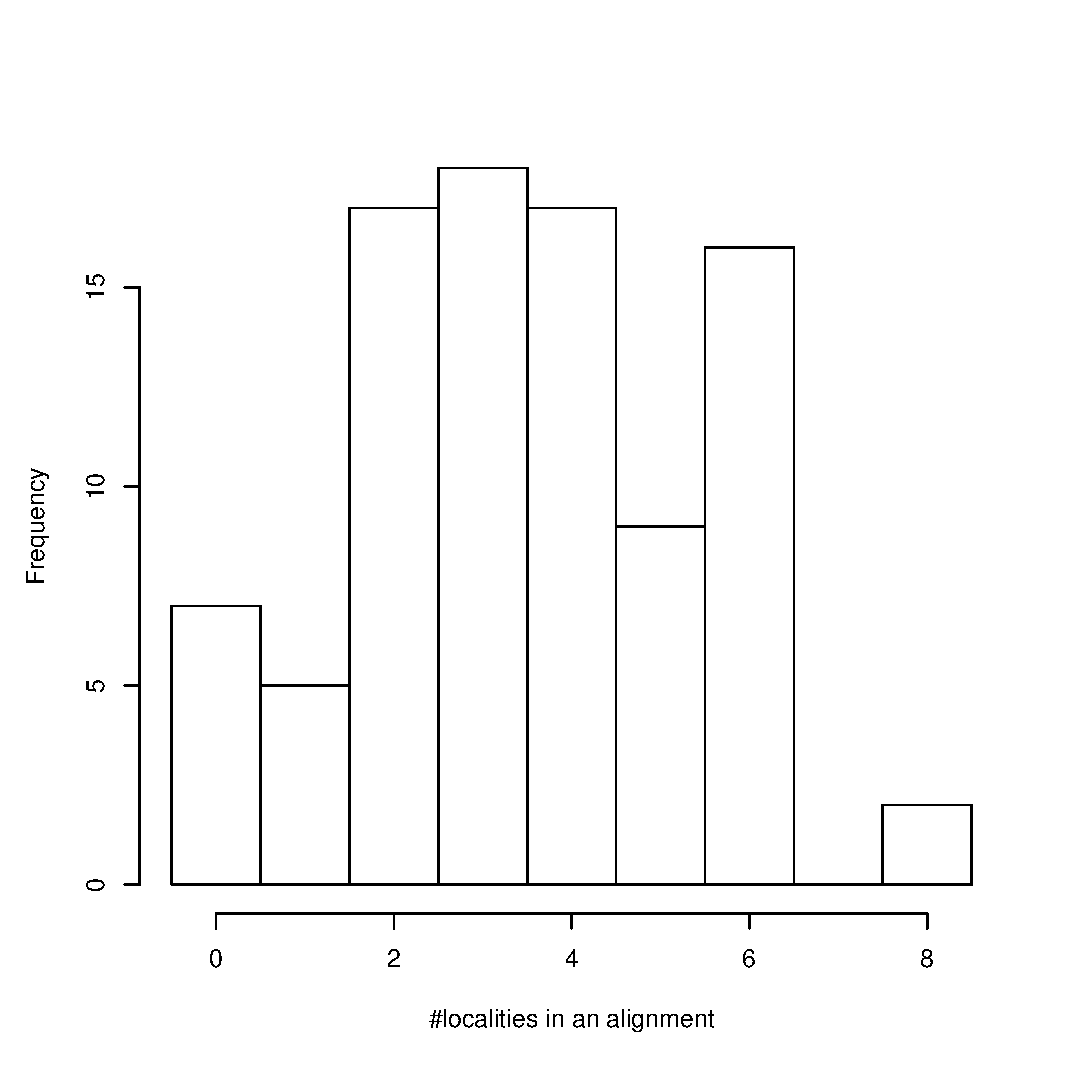
\includegraphics[width=0.9\columnwidth]{localitiesDistribution.eps}
  \end{center}
  \caption{Frequency distribution of the number of local ends in the
      in the data set of benchmark alignments. Only a small fraction of the
      alignments is global, while most test alignments have 2--6 local
      ends. }
  \label{fig:locs}
\end{figure}

These sequences are subsequently aligned with \SAFTWARE{} as well as three
of the most common alignment tools: \texttt{T-Coffee}
\cite{Notredame:00,Chang:14}, \texttt{MAFFT} \cite{Katoh:05,Nakamura:18},
and \texttt{ClustalW} \cite{Larkin:07,Sievers:18}. All three tools are
based on initial pairwise alignments and use essentially progressive
schemes, hence presenting efficient heuristics rather than exact solutions.

\begin{figure}
  \begin{center}
    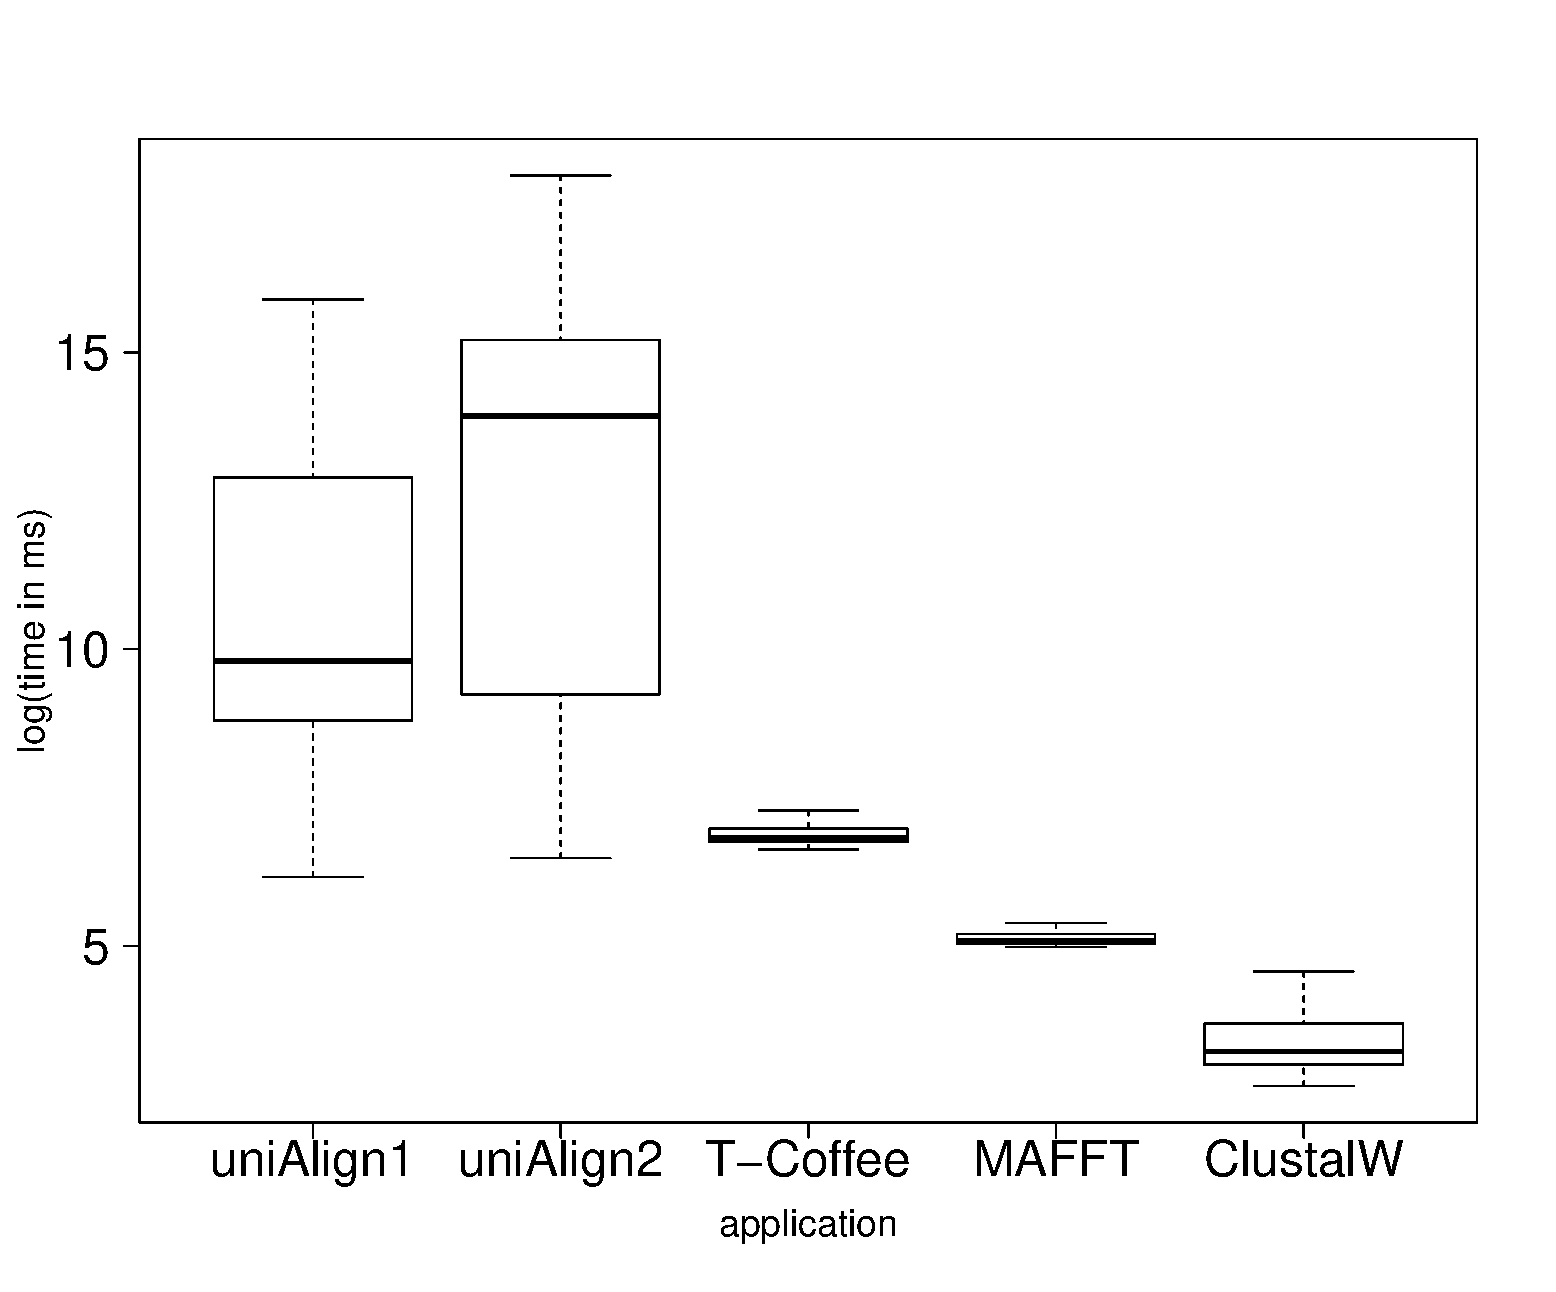
\includegraphics[width=1\columnwidth]{times_combined.eps}
  \end{center}
  \caption{Running time of \SAFTWARE{} for alignments with at most three
    local ends (\SAFTWARE$\le3$) and for alignments with more than three
    local ends (\SAFTWARE$>3$) compared to heuristic global aligners
    (\texttt{T-Coffee}, \texttt{MAFFT}, and \texttt{ClustalW}) that are
    commonly used in large-scale bioinformatics applications. \TODO{add
    discussion of the two implemented variants!}}
  \label{fig:manyLoc}
\end{figure}

Comparing the performance for few and many local ends, respectively, we can
see in Fig.~\ref{fig:manyLoc} that the running time of \SAFTWARE, as
expected, strongly depends on how many local ends needs to be handled in
one alignment. Without local ends, i.e., for global alignments, the
execution time of \SAFTWARE{} is comparable with \texttt{T-Coffee}. For
partially local alignments we observe the expected exponential increase
with the number of local ends. Since \SAFTWARE{} is designed as a reference
implementation of a much more expensive, exact algorithm, it is clear that
it cannot be competitive in terms resource consumption.
\TODO{Figure~\ref{fig:manyLoc} also compares the resource consumption for
  Eqs.~(\ref{eq:maxrec}) and (\ref{eq:maxrec2}). We observe that ***** }
Much more interesting than the comparisons of running times, however,
  is the question whether exact multi-way alignments yield an improvement
  in accuracy.

\begin{figure}
  \begin{center}
    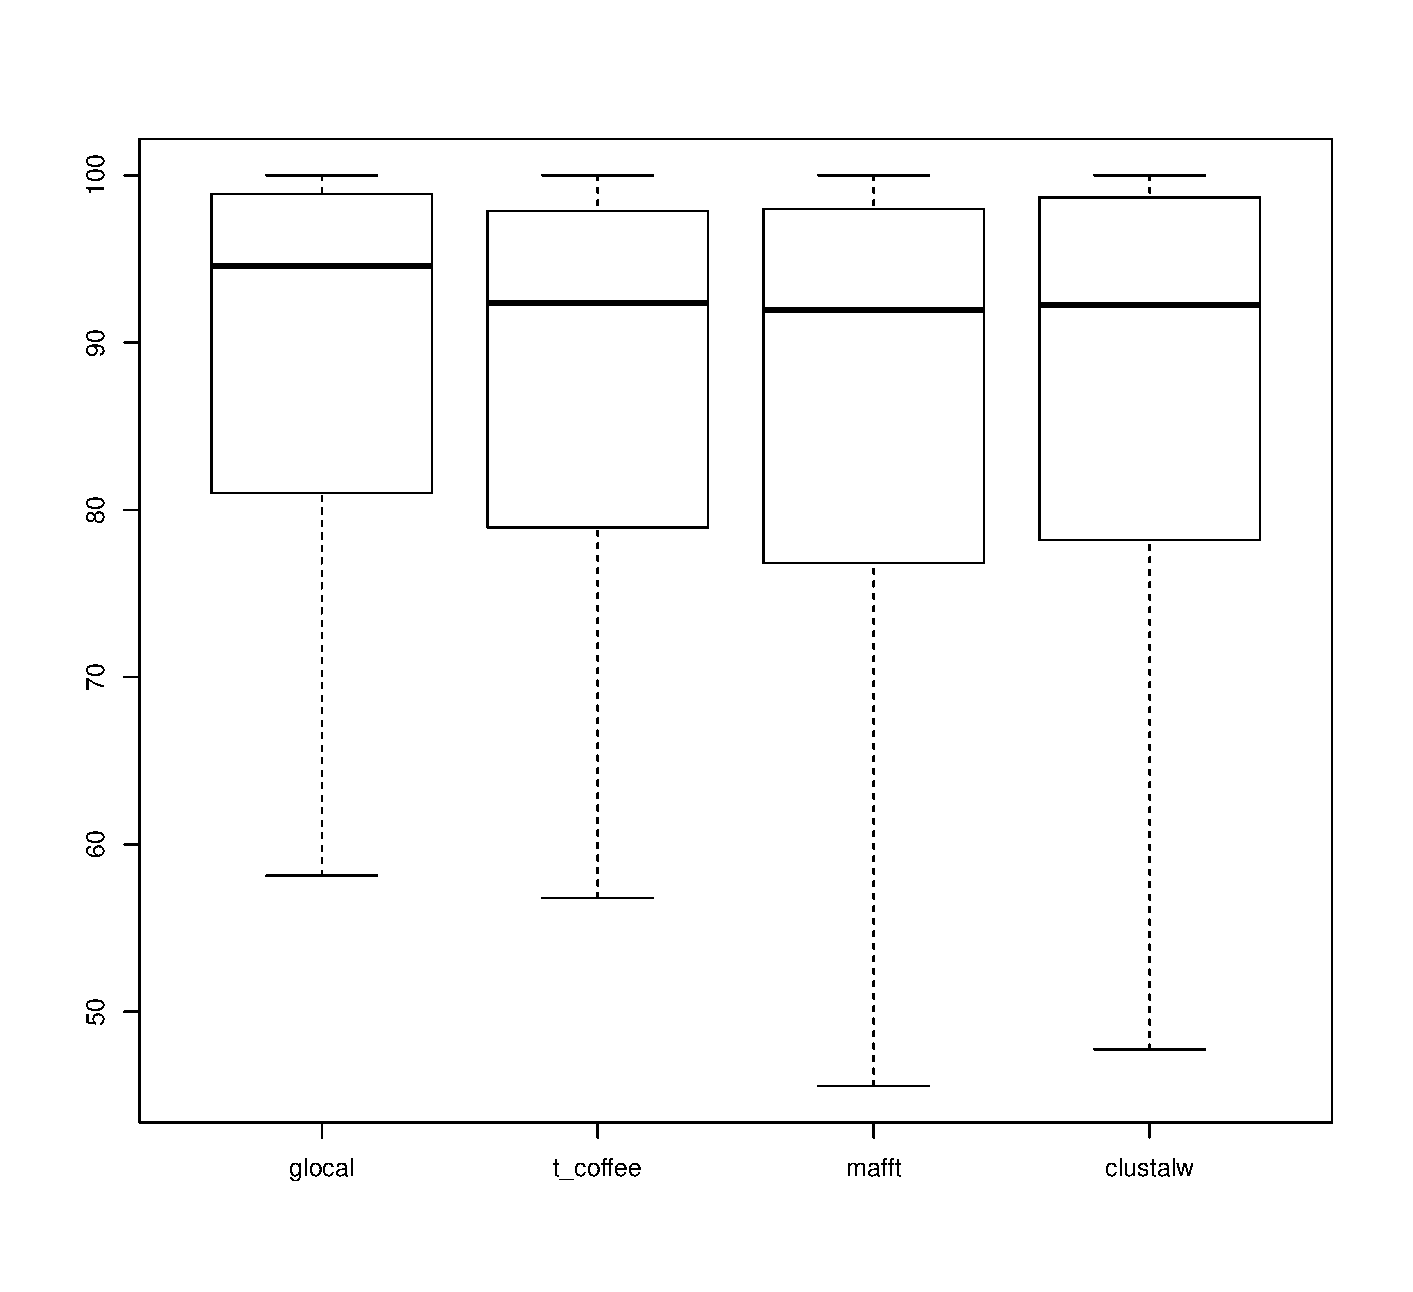
\includegraphics[width=1\columnwidth]{ac.eps}
  \end{center}
  \caption{Accuracy of \SAFTWARE{} compared to the heuristic global
    alignment tools \texttt{T-Coffee}, \texttt{MAFFT}, and
    \texttt{ClustalW}.}
    \label{fig:ac}
\end{figure}

The average accuracy, defined as $\mbox{AC}=(L-f)/L$ where $L$ is the
length of the alignment and $f$ is the number of columns deviating from the
reference alignment, is summarized in Fig.~\ref{fig:ac}. The data show that
\SAFTWARE{} provides a moderate but noticeable improvement relative to all
three heuristics, although we use a simple scoring model and none of the
protein-specific rules implemented e.g.\ in \texttt{ClustalW}.

\begin{figure}
  \begin{center}
    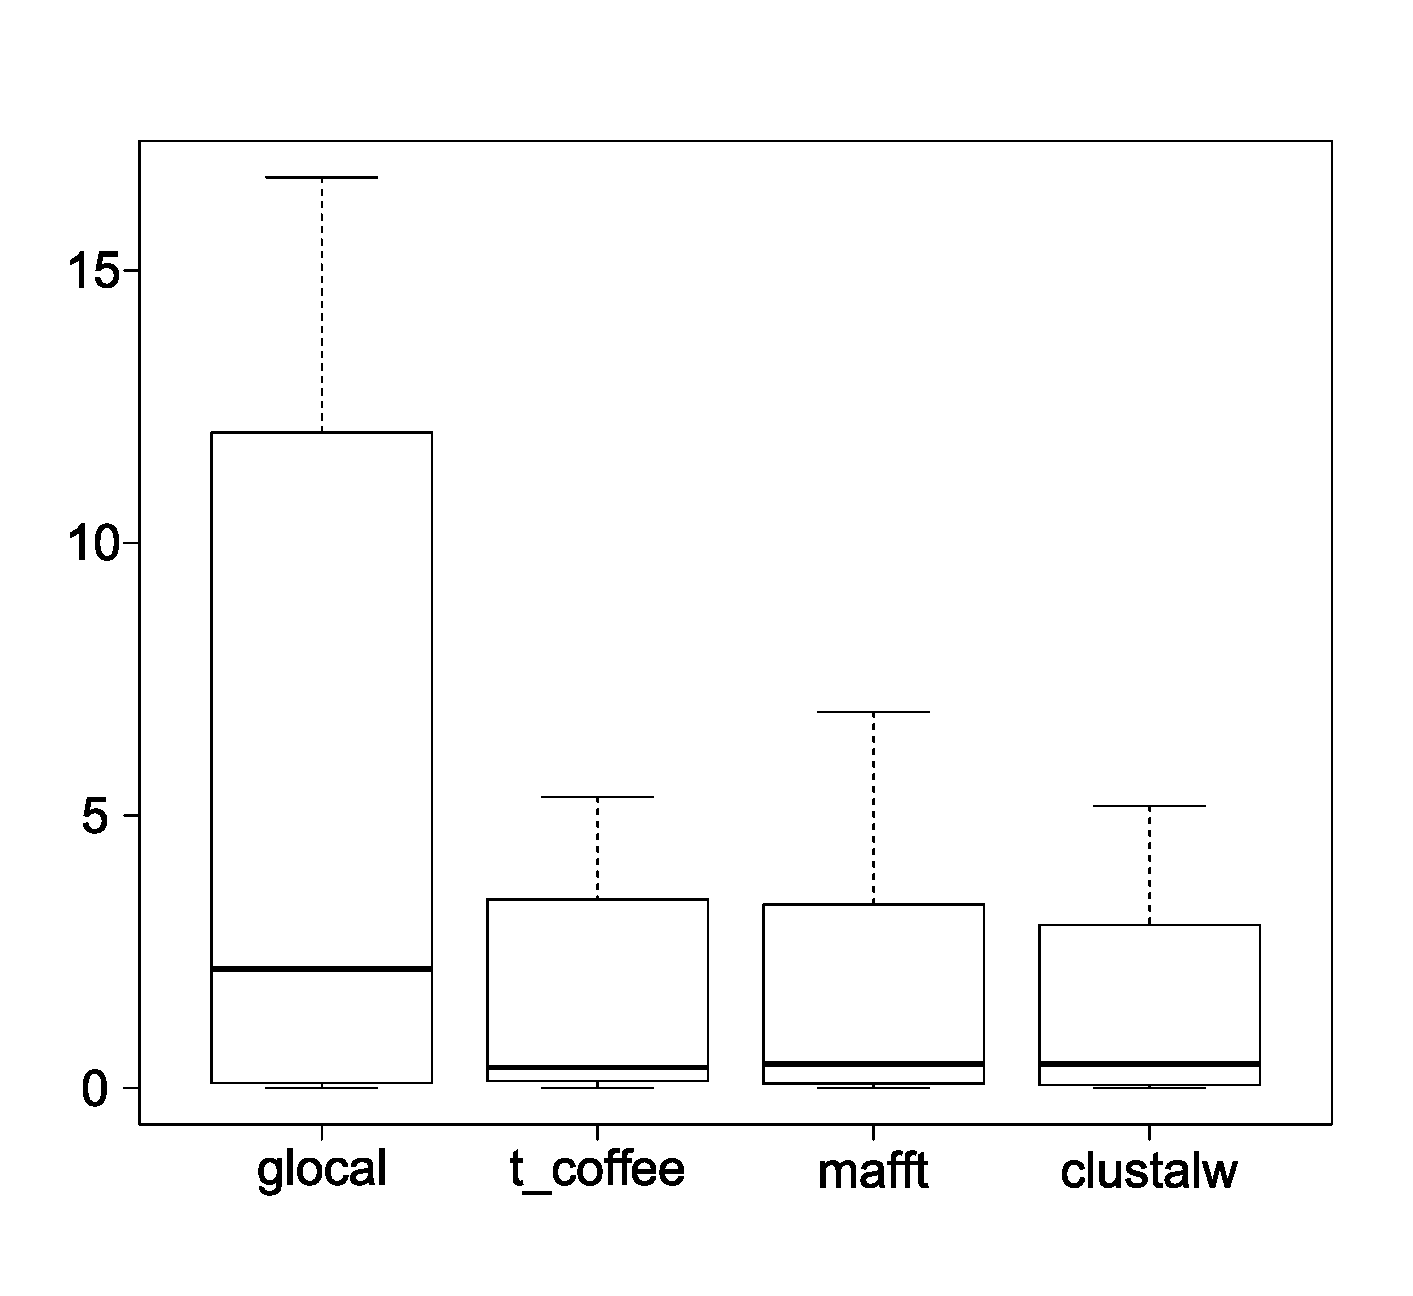
\includegraphics[width=1\columnwidth]{pse.eps}
  \end{center}
  \caption{Position shift error of \SAFTWARE{} compared to the heuristic
    global aligners \texttt{T-Coffee}, \texttt{MAFFT}, and
    \texttt{ClustalW}.}
  \label{fig:pse}
\end{figure}

The position shift error $\mbox{PSE}$ as defined by \citet{oxbench} serves
as an alternative measure of alignment accuracy. Consider a pair of
(mis)matched positions $i$ in sequence $x$ and $j$ in sequence $y$ in the
reference alignment. In the test alignment we consider the same position
$i$ in $x$ and its (mis)matched position $j'$ in $y$ and measure the
distance $\delta=|j-j'|$. A similar rule is used to compute $\delta$ if
there is an in/del between $x$ and $y$ at position $i$. For the details we
refer to \cite{oxbench}. The $\mbox{PSE}$ is the average of the
contributions $\delta$ of all mismatched pairs in the reference alignment.
Omitted prefixes and suffixes at local ends do not enter the $\mbox{PSE}$
score. \SAFTWARE{} exhibits significantly smaller position shift errors
than the three heuristics, Fig.~\ref{fig:pse}.

\section{\uppercase{Discussion}}

\SAFTWARE{} is primarily intended as a reference implementation against
which specialized partially local alignments can be tested and
benchmarked. We anticipate at least two use cases. First, \SAFTWARE{} is
useful to to create test cases and help debugging during the development
phase of a specialized exact implementation. More importantly, since
\SAFTWARE{} computed exact solutions for a moderate number of input
sequences, it can be used to generate ground-truth data against which
faster heuristics can be compared. The current version of \SAFTWARE{} was
not implemented to yield good performance while we expect that substantial
gains can be achieved by parallelization with fine grained multithreading
\cite{Martins:01}. Still it will need to be tested whether such a solution
is realizable in \texttt{Java}.

While biological sequences tend to be rather long as compared to average
word lengths we see a promising application to alignment of lexical items
where prefixing and suffixing seem to play even a bigger role that in
biology. Even though affixes can contain information, the root of words is
most valuable when doing cross-linguistics comparisons. For conceptual
examples we refer to \cite{Retzlaff:18a}.

The computational efforts for exact dynamic programming algorithms
  often can be reduced excluding subsets of matches using bounds on the
  achievable scores. Lossless filters for local pairwise alignments have
  been pioneered by \citet{Peterlongo:08,Peterlongo:09}. Ideas to prune the
  search space of the DP problem are discussed e.g.\ by
  \citet{Schroedl:05} or \citet{Bilu:06}.  Quasi-alignments based on $k$-mer matches
  can be employed as alignment anchors also in a global context
  \cite{Nagar:13}. These techniques may be used not only to reduce the
  computational effort of the exact algorithm for input sequences of
  practical interest, but also might serve as starting points for
  construcing efficient heuristics for partially local MSA problems.

The framework of \SAFTWARE{} lends itself to further extensions. First, it
is easily possible to derive a probabilistic version. This essentially
entails a change in the scoring from adding score contributions to
multiplying with the corresponding Boltzmann factors. The corresponding
outside algorithm could easily be constructed along the lines of
\citet{Hoener:15b}. Another extension that could be realized very easily is
to enforce additional constraints on state transitions. For example, it may
be useful in a pattern-based applications to allow the transition to and
from \textit{active} only concurrently, i.e., at the same position relative
to remaining input sequences.

Instead of treating state transitions in an acyclic manner, it is also
possible to allow multiple transitions from \textit{active} back to
\textit{inactive}. This would allow certain (context dependent) deletions
to occur at a unit cost. Such ``exclusions'' have rarely been considered in
sequence alignment but are of some interest for structured RNAs
\cite{Schirmer:13}. This idea may be of use in particular when sequences
are provided with structural annotation and deletions of entire structural
elements are to be scored in a special way.

Advances in computing technology now make it feasible to compute exact
simultaneous solutions of alignment problems with more than two
sequences. A combinatorial diversity of distinct alignment problems arises
in this setting just by allowing to distinguish local and global ends
separately for each input. We suspect that additional variations on the
theme are of interest, e.g., requiring additional constraints on pairwise
overlaps. The framework and the implementation presented here is a first
step towards an systematic exploration of this largely uncharted universe
of alignments, many of which we suspect will be of practical use in
computational biology.

\section*{\uppercase{Acknowledgments}}

NR gratefully acknowledges the hospitality of the Santa Fe Institute, where
parts of this work were performed, as well as travel support by the ASU-SFI
Center for Biosocial Complex Systems. The Competence Center for Scalable
Data Services and Solutions (ScaDS) Dresden/Leipzig is funded by BMBF grant
01IS14014B.

%\vfill
\bibliographystyle{apalike}
{\small
\bibliography{implementGLOCAL}}

\vfill
\end{document}
